\documentclass[conference]{IEEEtran}
\IEEEoverridecommandlockouts
\usepackage[ngerman]{babel}
% The preceding line is only needed to identify funding in the first footnote. If that is unneeded, please comment it out.
\usepackage{cite}
\usepackage{amsmath,amssymb,amsfonts}
\usepackage{algorithmic}
\usepackage{graphicx}
\usepackage{textcomp}
\usepackage{xcolor}
\usepackage{setspace}
\usepackage{booktabs}
\usepackage[export]{adjustbox}
\def\BibTeX{{\rm B\kern-.05em{\sc i\kern-.025em b}\kern-.08em
    T\kern-.1667em\lower.7ex\hbox{E}\kern-.125emX}}
\begin{document}

\title{Currency Exchange, eine App zur Anzeige von Wechselkursen mit Hilfe eines Webscrapers}


\author{\IEEEauthorblockN{1\textsuperscript{st} Matz, Annika}
\IEEEauthorblockA{
Berlin, Deutschland \\
s\_matz22@stud.hwr-berlin.de}
\and
\IEEEauthorblockN{2\textsuperscript{nd} Liebenberg, Benjamin}
\IEEEauthorblockA{
Oranienburg, Deutschland \\
s\_liebenberg22@stud.hwr-berlin.de}
\and
\IEEEauthorblockN{3\textsuperscript{rd} Reetz, Tobias}
\IEEEauthorblockA{
Berlin, Deutschland \\
s\_reetz22@stud.hwr-berlin.de}
%Beispiel wie es aussah
%\and
%\IEEEauthorblockN{3\textsuperscript{rd} Given Name Surname}
%\IEEEauthorblockA{\textit{dept. name of organization (of Aff.)} \\
%	\textit{name of organization (of Aff.)}\\
%	City, Country \\
%	email address or ORCID}
}

\maketitle


\section{Einführung}
Innerhalb unseres dualen Studiums der Informatik an der "Hochschule für Wirtschaft und Recht", nahmen wir an dem Modul Software-Engineering 2 teil. Ziel dieses ist die Entwicklung von Software, vermittelt zu bekommen und das erlernte Wissen direkt anwenden zu können innerhalb einer Projektarbeit. Dabei wird auf die Grundlagen des Projektmanagments geachtet, wofür z.B. UML-Diagrammen angefertigt werden. Zur Dokumentation des Projektes wird dieses Paper angefertigt. 
Innerhalb des Moduls werden auch Softskills gefördert, z.B. die Präsentationsfähigkeiten oder die Sozialkompetenz innerhalb von Gruppenarbeiten.

\section{Idee des Projektes}
Ein sehr großer Teil unseres Lebens dreht sich um das erwerben von unterschiedlichen Materiellen Gütern. Für unserer Arbeit werden wir vergütet, im Supermarkt kaufen wir davon unser Abendessen und an den Wochenenden und im Urlaub gehen wir auf Reisen. Auf diesen müssen wir uns in einer fremden Kultur zu Recht finden und konsumieren weiter Güter. Doch wie können wir einen Wert von diesen einschätzen, wenn wir die Währung nicht kennen? Und genau dieses Problem löst unsere App "Currency Exchange". Einfaches nachschlagen von tagesaktuellen Wechselkursen und umrechnen zwischen verschiedenen Währungen. Ein besonderes Feature ist das Umwandeln des eingegebenen Wertes in die Anzahl von Döner, welche damit gekauft werden könnten in Euro. \\
Die  Android-App arbeitet mit Hilfe eines Webscrapers, welcher Wechselkurse erhält.
% und Beträge der unterschied- lichen Währungen ineinander umrechnet.

\section{Projektorganisation}
Innerhalb eines Softwareentwicklungsprojekts erhalten die einzelnen Bearbeitenden verschiedene Rollen, die ihnen unterschiedliche Aufgaben zu teilen. In diesem Fall bestand das Entwicklungsteam aus wenigen Personen, so wurden keine expliziten Arbeitsbereiche vergeben.  So wurden Aufgaben nach und nach vergeben, wobei jeder Bereich eine eigene Ansprechperson besaß. Unterteilt wurde in Projektleitung, Serveradministration, Design und Testdurchführung. Zu Anfang wurde für essentiell wichtige Themen, wie z.B. die Software-Architektur oder den groben Design-Entwurf, wurden Teammeetings durchgeführt und die Umsetzung so zusammen geplant. Sichergestellt wurde so, dass jedes Teammitglied mit einbezogen wird und alle auf dem gleichen Stand sind. \\
Die Programmierung der Software wurde von Teammeeting zu Teammeeting aufgeteilt. Hauptsächlich kümmerten sich Benjamin und Tobias Reetz um die Programmierung des Webscrapers, sowie die Schnittstelle und ein Teil des Backend der App. Annika Matz kümmert sich vor allem um die Umsetzung des Designentwurfs zu einem funktionierenden Frontend, sowie ein Teil der Programmierung des Backend.

\subsection{Projektleitung}
Der Projektleitung wurde von Annika Matz übernommen. Unteranderem behielt sie die unterschiedlichen Abgabetermine im Blick. Außerdem sorgte sie für regelmäßig Treffen in der Gruppe und leitete diese an. Bei diesen wurde der aktuelle Stand ausgewertet, weitere Entwicklungsschritte besprochen und Aufgaben verteilt. \\
Des weiteren achtete sie auch auf die Projektanforderungen und führte die Qualitätssicherung durch, wodurch sie für eine angemessene Feedback innerhalb der Teammeetings sorgt.

\subsection{Serveradministration}
Der Bereich Serveradministration wurde von Benjamin Liebenberg beaufsichtigt. Aufgrund seiner weitreichenden Erfahrung in diesem Gebiet, konnte er diesen Bereich übernehmen. Er hostet unseren Webscraper auf seinem Server, sorgt für täglich aktualisierte Daten innerhalb der App und stellt die Schnittstelle für unsere App bereit.

\subsection{Design \& Testplanung}
Das Design und die Testplanung wurden zum größten Teil von Tobias Reetz übernommen. Aufgrund seiner Designerfahrung im Modul Software-Engineering 1, übernahm er diese Rolle und designte vor allem das App-Logo. Er sorgte für eine angemessene Farbgebung und dafür, dass die App aufgrund ihrer Gestaltung schnell wieder erkennt werden kann. \\
Außerdem übernahm er das Konkretisieren von Usability-Tests, welche wir zuvor im Plemnum entworfen hatte und führte diese mit unseren Kommilitonen durch. Damit trug er einen entscheidenen Beitrag zur Fehlersuche und somit zur Qualität unseres Programmes bei.

\section{Anforderungen}
An eine Software werden immer unterschiedliche Erwartungen und Anforderungen gestellt. Eine genaue Definition sind wichtig für den Erfolg des Projektes. In diesem Projekt werden die unterschiedlichen Anforderung in drei Kategorien unterteilt. Sie beinhalten nicht funktionale, funktionale und optionale funktionale Anforderungen.

\subsection{Nicht funktionale Anforderungen}
Nicht-funktionale Tests decken alle Anforderungen ab, welche das gesamte System ansich betreffen. Es werden somit keine Funktionen abgeprüft, sondern Eigenschaften und Bestandteile. Für das Projekt wurde besonders auf eine sehr gute Usability geachtet, was besonders durch eine intuitive und einfache Benutzung begründet werden soll.
Desweiteren soll eine Verfügbarkeit des Projekt auf Android-Handys garantiert werden. Um einen hohen Datenschutz garantieren zu können erheben wir keine Daten und speichern auch nicht die in der Vergangenheit getätigten Eingaben dem Nutzer zur Verfügung. 

\subsection{Funktionale Anforderungen}
Funktionale Anforderung definieren die Funktionen und Erwartungen der Software, welche für ein erfolgreiches Projekt erfüllt werden müssen. \\
Das wichtigste Ziel für die Software ist eine lauffähige Android-Handy-Applikation, welche verschiedene Eingaben zwischen verschiedenen Währungen richtig Umrechnen kann. Es soll immer ein tagesaktueller Wechselkurs bereit stehen. In die App sollen auch mindestens sieben Währungen eingebunden werden.

\subsection{Optionale funktionale Anforderungen}
Anforderungen, welche nicht essentiell notwendig für die grundlegenden Funktionsweise sind, aber sie diese erweitern, werden zu den optionalen funktionalen Anforderungen gezählt. \\
Zu diesen zählt die Umrechnung der Anzahl an Döner, die die Nutzenden sich mit dem eingetragenen Wert kaufen könnten in Euro. Außerdem könnte die App durch eine Funktion zum Hinzufügen von Prozentualen Werten ergänzt werden. Diese könnten zum Beispiel zur Berechnung der Mehrwertsteuer oder des Trinkgeldes genutzt werden.

\section{Entwurf}
Innerhalb eines Entwurfs wird der Aufbau und die Struktur des Projektes geplant und fest gehalten. Dieser besteht in diesem Projekt aus drei verschiedenen Komponentne der Systemarchitektur, einem Sequenzdiagramm und dem groben Designentwurf der Applikation. Diese Vorgaben dienen als Leitfaden für die Entwicklung der Anwendung.

\subsection{Systemarchitektur}
Die Systemarchitektur beschreibt die Struktur des Projektes, vorhandenen Komponenten und unterschiedlichen Bereiche, während sie zusätzlich erklärt wie diese miteinander interagieren. 
Currency Exchange’s Systemarchitektur besteht aus den zwei Bereichen User-Client und Server. Da hier nur zwei Bereiche existieren handelt es sich um eine Zwei-Tier-Architektur, weil es einen Applikationsbereich also den User-Client und einem Back-End- bzw. Datenbankbereich dem Server besteht.\\
Der User-Client enthält die Business-Logik, welche durch die zwei Unterkategorien View, welcher dabei die Benutzeroberfläche darstellt, und Controller, der für die Verarbeitungslogik die Verantwortung trägt, aufgebaut ist. Der View besteht aus dem Header, der das Logo von Currency Exchange enthält und dem Knopf für den Dark-Mode, der Navigationsleiste, welche eine Übersicht über die verschiedenen Seiten anzeigt, und dem Inhalt, wo dann sämtliche Informationen und Interaktionen statt finden. Über die Interaktion mit diesen können Nutzende mit dem Controller interagieren, über den die unterschiedlichsten Funktionen ausgeführt werden können. Der Controller besteht hier auch wieder aus drei Komponenten. Die erste ist der Navigator, in ihm ist geregelt wie die bereitgestellten Daten formatiert werden sollen, damit sie für die Nutzenden im View beim Inhalt ordnungsgemäß dargestellt werden können. Ein weiterer Teil des Controllers ist der Calculator, welcher für sämtliche Umrechnungen zuständig, wofür er auch Anfragen an den Navigator schickt, um zu wissen welche Operation er durchzuführen hat, und an die letzte Komponente, dem Data-Manager, von dem er die entsprechenden Wechselkurse erfragt. Der Data-Manager ist für die Verarbeitung der Daten zuständig, wozu das Abspeichern, das Einlesen, das Aufarbeiten und Aktualisieren, wofür er per HTTP-Request Anfragen an den Server sendet, der Daten gehört.\\
Der Server beinhaltet auch einen Controller, der aus einem Bash-Skript und einem Data-Manager. Das Bash-Skript ist für den Webscraper verantwortlich, was bedeutet, dass es den Webscraper einmal am Tag aktiviert, welcher dann wiederum Daten aus dem Internet sammelt. Nach dem der Webscraper die Daten gesammelt hat, wird der Data-Manager aktiviert welcher dann diese aufarbeitet und in einer CSV-Datei bereit stellt, da sie eine einfaches Arbeiten durch ihre Strukturierung ermöglicht.\\
Durch die Einbindung des Webscraper auf einem externen Server, wird eine geringe Anfrage auf die Website mit den Wechselkursen garantiert. Denn sollten zu viele Anfragen an die Webseite geschickt werden, kann es zu einer Überlastung dieser kommen. Mögliche folgen wären das Abstürzen dieser Seite.

\subsection{Sequenzdiagramm}
Das Sequenzdiagramm ist für die graphische Darstellung der Kommunikation von den unterschiedlichen Instanzen innerhalb der Software und mit dem User verantwortlich. 
Das Diagramm ist in mehrere Bereiche untergliedert, welche der Serverbereich, Kommunikation von der Applikation und Server und der Interaktion mit dem User sind.
Der Server besteht aus verschiedenen Instanzen, die für die Funktionalitäten verantwortlich sind. Die erste Komponente ist der Webscraper, welcher zur Zweiten, der Webseite von der die Informationen bezogen werden, eine Anfrage schickt, woraufhin diese die Antwort mit sämtlichen Daten zurücksendet. Nach dem Erhalt des Webseiteninhalts, sortiert der Webscraper sämtliche Informationen und sendet sie an die dritte Instanz, welche die Wechselkursliste ist und die die sortierten Daten dann abspeichert.\\
Die Applikation ist eine Instanz innerhalb des Sequenzdiagramms, welches durch die zwei Teilinstazen dem Back- und Front-End vertreten wird und es für die letzten beiden Bereiche des Diagramms verantwortlich ist. Für den Ersten dieser Bereiche ist nur das Back-End verantwortlich, weil es an den Server, genauer gesagt an die Währungsliste, eine Anfrage sendet, mit der die aktualisierten Daten abgefragt werden sollen. Besteht eine Internetverbindung sendet die Liste die neuen Informationen an das Back-End, welches dann die Informationen intern abspeichert. Sollte jedoch keine Verbindung zum Internet bestehen wird mit den schon besthenden Daten der Applikation weiter gearbeitet.\\
Innerhalb des letzten Bereiches des Diagramms, welcher sich mit der Verarbeitung der der User-Inputs beschäftigt, spielen auch die Instanzen des Font-Ends und des Users eine Rolle. Der User hat diverse Möglichkeiten mit der Applikation zu interagieren, welche in die zwei Kategorien , die jeweils einen ähnlichen Aufbau aufweisen, der logischen und graphischen Anpassung unterteilt werden kann.  Bei der logistischen Komponente sendet der User eine von drei Nachrichten an das Back-End, welches dann eine Anfrage über die ausgewählten Werte an das Front-End sind. Die Userbefehle sind klickSwapSpinnerValues, welche die ausgewählten Währungen miteinander tauscht, selectCurrency, welche es ermöglicht eine neue Währung auszuwälen, und klickCalculateValues, welche die Werte berechnet. Nach dem Erhalt der Informationen des Front-Ends, führt das Back-End dann jeweils Funktionen aus, die die Werte tauschen, neue aus wählen oder den Wechselkurs und die Döneranzahl berechnen. Zum Schluss sendet es die Berechnungen zurück an das Front-End, welches daraufhin das Anzeigen dieser übernimmt. Die letzten drei Möglichkeiten, die der User hat, sind die graphischen Anpassen, bei denen entweder die Home-Seite  oder die FAQ-Seite angzeigt wird und zwischen Dark- und Light-Mode gwechselt werden kann. Dafür sendet der User eine Nachricht an das Front-End, welches dann die Veränderungen darstellt.

\subsection{grober Designentwurf}
\begin{figure}[h]
	\centering
	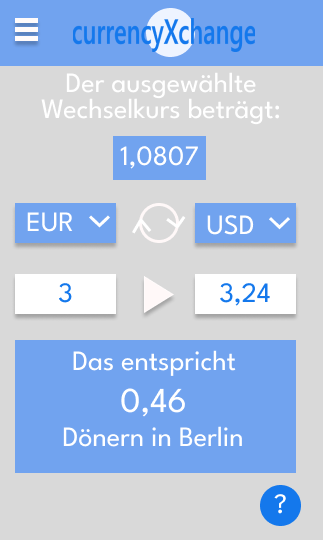
\includegraphics[width=0.5\linewidth, frame]{designentwurf}
	\caption[Designentwurf]{Designentwurf}
	\label{fig:designentwurf}
\end{figure}



\section{Implementierung}

\subsection{Konsistenz}

\subsection{Vorbereitung}
Innerhalb der Vorbereitungsphase werden wichtige Punkte für den Verlauf des Projekts festgelegt. Einer dieser Punkte ist die Versionsverwaltung. Über sie werden die verschiedenen Stände der Software gesteuert und überblickt. Außerdem kann im Fall von irreversiblen Fehlern auf frühere Versionen zugegriffen werden, wodurch es vermieden wird händisch den gesamten Code auf einen früheren Stand um zu strukturieren, was bei großen Codemengen sehr zeitaufwändig ist und somit viel Zeit der Bearbeitung einspart. Dazu wurde die Plattform GitHub verwendet, weil sie verständlich gestaltet worden ist und somit wenig Zeit für die Einarbeitung benötigt. Zu dem ist GitHub kostenfrei und weit verbreitet, was bei Problemen mit der Versionsverwaltung zu einem breiten Angebot von Hilfestellungen führt, da wahrscheinlich das Problem schon irgendwann mal aufgetaucht ist.\\
Ein weiterer Punkt ist die Namenskonvention von Funktionen, Variablen und Dateien. Hierbei wurde festgelegt, dass die Namen deskriptiv sein sollen, damit sie möglichst einfach zu verstehen sind. Deskriptive Namen werden so gestalten, dass der Namen alleine die Funktionalität beschreiben kann, wodurch auch viele Kommentarzeilen eingespart werden können, weil der Name diese Funktion schon übernimmt und eine genauere Beschreibung selten benötigt wird.\\
Der wichtigste Punkte innerhalb eines Softwareprojekts sind die verwendete Entwicklungsumgebung und verwendeten Programmiersprachen. Da das Ziel bei Currency Exchange durch eine Android-App dargestellt wird, wurde nach einer Entwicklungsumgebung gesucht, die den Entwicklungsprozess durch Verbesserungsvorschläge und graphische Darstellungen der Applikation unterstützt. Eine solche Entwicklungsumgebung ist Android-Studio verwendet, weil sie ohne weitere Einstellungen Codeverbesserungen vorschlägt und einen eingebauten Emulator besitzt, der es vereinfacht die Anwendung graphisch wahrzunehmen, zu simulieren und Fehler während der Laufzeit zu finden. Dies wird des Weiteren auch durch die Namensgebung unterstrichen. Innerhalb von Android-Studio besteht die Möglichkeit zwischen den zwei Programmiersprachen Kotlin und Java zu wählen, welche beide Objekt orientierte Sprachen sind. Durch die bereits vorhandenen Vorkenntnisse des Projektteams mit der Programmiersprache Java, wurde sie als Entwicklungssprache ausgewählt, weil somit die Einarbeitungszeit in eine neue Sprache eingespart werden konnte und direkt mit der Entwicklung der Applikation begonnen werden konnte.

\section{Integration}
Die Integration in der Softwareentwicklung beschäftigt sich mit den Schnittstellen zwischen den unterschiedlichen Systemkomponenten und der Testung dieser, da es wichtig ist, dass diese miteinander kompatibel sind und bei den Übertragungen der zwischen Komponenten keine Fehler auftreten. Hierzu stehen den entwickelnden Personen diverse Methoden zur Verfügung, von denen eine die Top-Down Integration ist, welche sich dadurch kennzeichnet, das obere Schichten zu erst integriert und die unteren Schichten durch Simulationen dargestellt werden, wodurch die Grundfunktionalitäten erst einmal getestet und validiert werden können, bevor dann im darauffolgenden Schritt die Komponenten zusammengeführt und erneut überprüft werden.\\
Im Fall von Currency Exchange bedeutete dies, dass im ersten Schritt der User-Client, welcher mit Hilfe von fest eingebauten Werten getestet wurde, und der Webscraper, der die CSV-Datei über einen Port zugänglich macht und überprüft wurde, ob alle Daten richtig sortiert wurden, integriert. Im zweiten Schritt wurde die beiden Komponenten zusammen geführt und bildeten ein neues System, welches dann erneut überarbeitet und getestet worden ist. 
%TODO Big Bang

\section{Tests}
Um zu validieren, dass die Software in ihren Funktionen korrekt ist, muss diese ausreichend getestet werden. Dazu müssen die Funktionen, die Persistenz und die Handhabung überprüft werden. Um dies zu bewerkstelligen, wird von Testmethoden Gebrauch gemacht. Da es jedoch kaum möglich ist, alle Bestandteile der Software gleichzeitig zu testen, wird die Überprüfung in mehrere Schichten unterteilt.\\
Vor allem während der Implementierungsphase, also der eigentlichen Entwicklung der Applikation, wird hierzu auf das Experience-based Testing zurückgegriffen. Dabei werden die geplanten Funktionen standardmäßig implementiert und anschließend auf Korrektheit getestet. Vorteil dieser Testmethode ist es, dass die Funktionen und Hintergrundprozesse bekannt sind. Somit kann der Entwickler Fehler direkt ausfindig machen und möglichst unmittelbar an der Behebung dieser arbeiten.\\
Jedoch birgt diese Testmethode auch Risiken. Schließlich kann es vorkommen, dass Fehler in früheren Implementierungen entstehen, die womöglich beim Testen der neuen Funktionalitäten nicht auffallen. Aus diesem Grund wurde während der Erstellung der Software zusätzlich auf das sogenannte Beta-Testing zurückgegriffen. Dabei wird die Software von Personen getestet, welche mit den Funktionen und der Benutzeroberfläche nicht vertraut sind. Dadurch kann es zu einer Fehlbedienung kommen, welche aus Sicht der Entwickler:innen im schlechtesten Falle zu einem Absturz des Programms führt, im besten Fall nur einen Fehler auswirft. Außerdem füllen die Personen nach dem Testen der Applikation einen kurzen Fragebogen aus, welcher vor allem die Dokumentation der Fehler und Anregungen für etwaige Verbesserungen zum Thema hat. Sinngemäß beinhaltet das Beta-Testing also die Testmethoden für die Benutzerfreundlichkeit (eng. usability-tests), als auch für die Funktionalitäts-Tests (Black-Box-Testing).
Mit diesen gewonnen Daten kann die Anwendung anschließend verbessert  und mögliche Fehler beseitigt werden. \\
Im Fall von Currency Exchange wurde ein Beta-Test am 13.03.2024 durchgeführt, welcher aufschlussreiche Informationen über die Verbesserung der Applikation geliefert hat. Beispielsweise wurden einige Fehler gefunden, die den Absturz der Software zur Folge hatten. Außerdem wurden Anregungen hinsichtlich der Benutzeroberfläche und Bedienung getätigt, welche eine Überarbeitung des Designs zur Folge hatten.

\section{Wartung}

\section{Rollout}

\section{Ergebnis}

Die entwickle Software läuft komplikationslos und erfüllt alle Grundanforderungen, sowie vereinzelt optionale funktionale Anforderungen. Darunter fällt die Berechnung in Döner.  Das Abziehen bzw. Hinzufügen von prozentualen Anteilen konnte bedauerlicherweise nicht umgesetzt werden. Die Grundanforderung, dass min. 7 Währungen angeboten werden konnten wir bei weitem übertreffen.\\
Herausforderungen brachte vor allem das Design des Frontends der App. Innerhalb der Implementierung stellten wir fest, dass einige Funktionen fehlen oder aber auch zu viel sind. So kam über die weitere Entwicklung der App eine textliche Anzeige der umgerechneten Werte hinzu. Diese soll die Bedeutung der einzelnen Werte verdeutlichen und für eine bessere Verständlichkeit sorgen. Leider wurde aufgrund dieser Zustände die Benutzeroberfläche sehr voll, wodurch der Button mit dem Fragezeichen entfernt werden musste. Wir entschieden uns für dieses Element, da der Button nur eine Ergänzung zum Hamburger-Menü und der dortigen Seitennavigation gewesen ist. Von diesem wäre der Nutzer auch nur zur Informationsseite gekommen. \\
Verbessert werden könnte noch die Auswahl der Währung innerhalb der Spinner. Aufgrund einer einfachen Umsetzung konnten sehr viele Währungen angeboten werden. Dies führt leider jedoch zu einer sehr unübersichtlichen Liste, welche sehr lang ist. Zur Lösung könnte eine Suchfunktion implementiert werden, welche die begehrte Währung herausfiltert. Durch diese Erfahrungen konnte die Gruppe ihre Kompetenzen in der Front-End Entwicklung weiter aus bauen, welche zuvor nur bedingt vorhanden war.

\section{Abschluss}
Insgesamt konnte das Projekt erfolgreich abgeschlossen werden. Die Fähigkeiten innerhalb der Software Entwicklung konnten weiter vertieft und ausgebaut werden, sowie eine lauffähige Software entwickelt und alle erforderlichen Abgaben konnten getätigt werden.
Besonders gut verlief die Arbeit innerhalb der Teammeetings. Es war dauerhaft eine konstruktive Arbeitsatmosphäre, in welcher vor allem in der Phase der Konzeptionierung zielgerichtet diskutiert werden konnte. Auch während des Debuggens in der Gruppe konnte gemeinsam schnell fehlerhafter Code korrigiert werden. So konnten wir schnelle Ergebnis erreichen. \\
Vereinzelt traten Schwierigkeiten in der Kommunikation während der Implementierung auf. So entstanden Situationen, bei welchen die Gruppenmitglieder sich falsch verstanden oder nicht alle wichtigen Informationen zwischen ihnen transferiert werden konnten. Dies konnte jedoch durch die vielen Gruppenmeetings und Absprachen schnell behoben bzw. korrigiert werden, sodass sie zu keinem größeren Problem innerhalb der Gruppe führen konnten. Durch diese Erfahrungen konnten wir unsere Softskills innerhalb der Kommunikation untereinander verbessern.


\end{document}
